\section{例题与分析}

\begin{question}\begin{example}[沿圆弧缓慢提升]\label{em3:example:1}
质量$m$的物块沿固定光滑圆弧，由最低点$A$缓慢拉到与圆心等高的$B$，圆弧半径为$R$，拉力始终切向。分别用动能定理与力的位移积分求拉力功。
\end{example}
\fig{fig:em3:example:1:s}{题设：沿圆弧缓慢提升}{\begin{tikzpicture}[scale=.9]\draw[world](0,0)arc(-90:0:2);\fill(0,0)circle(.08)node[below]{$A$};\fill(2,2)circle(.08)node[right]{$B$};\draw[guide](0,0)--(0,2)--(2,2);\node[left]at(0,1){$R$};\end{tikzpicture}}
\end{question}
\begin{solution}\textbf{由高度差列动能定理}\par\nobreak
图\ref{fig:em3:example:1:s}的高度增加为$R$，不是直径$2R$。缓慢运动使初、末动能均可忽略，支持力不做功，故$W_F-mgR=0$，得到$\boxed{W_F=mgR}$。
\fig{fig:em3:example:1:p}{切线微位移只计入拉力与重力的切向分量}{\begin{tikzpicture}

\coordinate(O)at(0,2.5);\coordinate(P)at(1.768,.732);
\draw[world](0,0)arc(-90:0:2.5);\draw[guide](0,0)--(O)--(P);
\fill(O)circle(.04)node[above]{$O$};\fill(P)circle(.07)node[below right]{$P$};
\draw[force](P)--++(.9,.9)node[right]{$F$};\draw[force](P)--++(0,-1.2)node[below]{$mg$};
\draw[force](P)--++(-.8,.8)node[left]{$N$};
\draw[->,blue](2.268,.232)--(2.868,.832)node[right]{$\dd s=R\dd\phi$};
\draw(0,1.8)arc(-90:-45:.7);\node at(.3,1.5){$\phi$};
\node[align=left]at(4.9,.2){$F=mg\sin\phi$\\$N\perp\dd\bm r$};
\end{tikzpicture}}

若初、末仍保留相同的很小速率，动能差也趋于零，因此这里的“缓慢”可以理解为准静态极限。圆弧支持力与切线位移垂直，功为零；重力功只由升高$R$决定，为$-mgR$。这样动能定理中的每一项都有明确的作用力与符号。



\par\medskip\Needspace{4\baselineskip}\noindent\textbf{沿圆弧积分切向拉力}\par\nobreak
在图\ref{fig:em3:example:1:p}中以最低点半径为转角起点，$0\le\phi\le\pi/2$，弧长微元$\dd s=R\dd\phi$。切向平衡给$F=mg\sin\phi$，于是
\[
W_F=mgR\int_0^{\pi/2}\sin\phi\dd\phi
=mgR[-\cos\phi]_0^{\pi/2}
=mgR(0+1)=mgR.
\]
两种方法分别使用始末状态与局部力，说明功的积分只累计切向分量。若拉到圆的最高点，高度差变成$2R$，功也相应变为$2mgR$。\end{solution}
\begin{question}\begin{example}[弹簧小球下落到竖直位置]\label{em3:example:2}
弹簧一端固定于$O$，自然长$\ell_0$、劲度系数$k$，另一端连质量$m$的小球。球从与$O$等高、弹簧自然长的位置$A$静止释放。到$O$正下方$B$时，弹簧伸长$\ell_0/n$，其中$n>0$。求该瞬间速率，并说明所得表达式的必要条件。
\end{example}
\fig{fig:em3:example:2:s}{初态弹簧水平且为自然长，末态位于悬点正下方}{\begin{tikzpicture}

\coordinate(O)at(0,2.4);\draw[spring](O)--(2.5,2.4);\fill(O)circle(.05)node[above left]{$O$};
\fill(2.5,2.4)circle(.08)node[right]{$A,\ v_A=0$};\node[above]at(1.25,2.4){$\ell_0$};
\draw[spring](O)--(0,-.7);\fill(0,-.7)circle(.08)node[below]{$B$};
\draw[dim](-.65,2.4)--(-.65,-.7)node[midway,left]{$\ell_0(1+1/n)$};
\node[right]at(.4,.8){末态伸长量：$\ell_0/n$};
\end{tikzpicture}}
\end{question}
\begin{solution}\textbf{区分下降高度与弹簧伸长}\par\nobreak
按图\ref{fig:em3:example:2:s}，球下降的高度等于末端弹簧长度$\ell_0(1+1/n)$，弹簧伸长量才是$\ell_0/n$。重力做正功，弹力做负功，故
\[mg\ell_0\left(1+\frac1n\right)-\frac{k\ell_0^2}{2n^2}=\frac12mv_B^2.\]
\fig{fig:em3:example:2:p}{重力功使用整个下降高度，弹力功使用相对自然长的伸长量}{\begin{tikzpicture}

\draw[guide](-.3,2.5)--(3.2,2.5);\fill(0,2.5)circle(.05)node[above]{$O$};
\draw[spring](0,2.5)--(0,-.5);\fill(0,-.5)circle(.09)node[below left]{$B$};
\draw[guide](-.3,.25)--(3.2,.25);\node[right]at(3.2,.25){自然长端点高度};
\draw[dim](.7,2.5)--(.7,.25)node[midway,right]{$\ell_0$};
\draw[dim](.7,.25)--(.7,-.5)node[midway,right]{$\ell_0/n$};
\draw[dim](2.6,2.5)--(2.6,-.5)node[midway,right]{$h=OB$};
\draw[force](0,-.5)--(-.0,.1)node[left]{$k\ell_0/n$};\draw[force](0,-.5)--(0,-1.6)node[below]{$mg$};
\node[align=left]at(6.2,1.2){$W_g=mgh$\\$W_k=-k(OB-\ell_0)^2/2$};
\end{tikzpicture}}



\par\medskip\Needspace{4\baselineskip}\noindent\textbf{求速率并检查状态是否可能达到}\par\nobreak
把方程两边乘$2/m$，得$v_B^2=2g\ell_0(1+1/n)-(k/m)(\ell_0/n)^2$。第一项使用球的下降高度，第二项使用弹簧相对自然长的形变量；两种长度不能相互替换，图中$OB$和$OB-\ell_0$分别承担这两个角色。

由图\ref{fig:em3:example:2:p}的能量转化得到
\[\boxed{v_B=\sqrt{2g\ell_0(1+1/n)-k\ell_0^2/(mn^2)}}.\]
弹簧长度可以变化，穿过竖直线时速度未必水平；本题只求速率，无须另加刚性摆的切向约束。根号非负是该状态可能出现的必要条件，但不是任意$n$都能由同一初态实际达到；$n$应由真实轨迹在穿过竖直线时的伸长确定。不能把给定的末态伸长当成独立可任意调整的运动参数。\end{solution}
\begin{question}\begin{example}[两物块被弹簧推开]\label{em3:example:3}
光滑水平面上，弹簧左端固定，右端连质量$m_A$的物块$A$。将弹簧压缩$x_1$，再把质量$m_B$的物块$B$紧贴放在$A$右侧，两块不粘连。由静止释放，求$A$相对初始位置向右运动的最大距离。
\end{example}
\fig{fig:em3:example:3:s}{以弹簧连接点的自然长位置为位移零点}{\begin{tikzpicture}

\draw[world](0,-.3)--(0,1.1);\draw[world](0,0)--(5.6,0);
\draw[spring](0,.4)--(1.8,.4);\draw[world](1.8,0)rectangle(2.6,.8);\node at(2.2,.4){$A$};
\draw[world](2.6,0)rectangle(3.4,.8);\node at(3,.4){$B$};
\draw[guide](3.8,-.5)--(3.8,1.25);\node[above]at(3.8,1.25){自然长连接点};
\draw[dim](1.8,-.45)--(3.8,-.45)node[midway,below]{$x_1$};
\end{tikzpicture}}
\end{question}
\begin{solution}\textbf{用接触力判定自然长处分离}\par\nobreak
图\ref{fig:em3:example:3:s}中弹簧压缩时，两物块共同向右加速。弹簧到自然长前接触力为正；到自然长时弹簧力变为零，之后若仍接触就需$B$拉住$A$，这是不可能的，故在自然长处分离。由共同运动段的动能定理
\[\frac12kx_1^2=\frac12(m_A+m_B)v_*^2,\quad v_*=x_1\sqrt{\frac{k}{m_A+m_B}}.\]
\fig{fig:em3:example:3:p}{先共同恢复自然长，再由物块A独自拉伸弹簧}{\begin{tikzpicture}

\foreach \yy/\xx/\title in {3.4/1.4/初始压缩,1.7/2.7/自然长分离,0/3.5/A首次停止}{
\begin{scope}[yshift=\yy cm]\draw[world](0,0)--(0,.9);\draw[spring](0,.35)--(\xx,.35);
\draw[world](\xx,0)rectangle++(.7,.7);\node at(\xx+.35,.35){$A$};\node[left]at(-.2,.35){\title};\end{scope}}
\draw[world](2.1,3.4)rectangle(2.8,4.1);\node at(2.45,3.75){$B$};
\draw[world](3.4,1.7)rectangle(4.1,2.4);\node at(3.75,2.05){$B$};
\draw[flow](2.8,2.7)--(4,2.7)node[midway,above]{$v_*$};
\draw[world](5,0)rectangle(5.7,.7);\node at(5.35,.35){$B$};\draw[flow](5.15,1)--(6.3,1)node[right]{$v_*$};
\draw[guide](2.7,-.4)--(2.7,4.5);\node[above]at(2.7,4.5){连接点$x=0$};
\draw[dim](1.4,-.5)--(2.7,-.5)node[midway,below]{$x_1$};\draw[dim](2.7,-.5)--(3.5,-.5)node[midway,below]{$x_2$};
\end{tikzpicture}}

在共同加速段设压缩量为$x>0$，有$a=kx/(m_A+m_B)$，$B$所受接触力为$N=m_Ba=m_Bkx/(m_A+m_B)>0$。到$x=0$时$N=0$；若继续令两块一起运动且$x<0$，就会得到$N<0$，这违反只接触、不粘连的条件。因此分离点由受力条件确定，不能仅凭弹簧恢复自然长的图形直觉判断。



\par\medskip\Needspace{4\baselineskip}\noindent\textbf{由A的独立运动求最远位置}\par\nobreak
图\ref{fig:em3:example:3:p}中$B$匀速离开，$A$独自拉伸弹簧。到$A$第一次停止时，$\tfrac12m_Av_*^2=\tfrac12kx_2^2$，所以$x_2=x_1\sqrt{m_A/(m_A+m_B)}$。从初始压缩位置算起
\[\boxed{s_{A,\max}=x_1+x_2=x_1\left(1+\sqrt{\frac{m_A}{m_A+m_B}}\right)}.\]
应把到自然长的$x_1$也计入位移。$m_B\to0$时最大位移趋于$2x_1$，与单个弹簧振子相符。\end{solution}
\begin{question}\begin{example}[阻力随深度增加的钉入过程]\label{em3:example:4}
钉子水平进入固定木板时受到阻力，大小为$F=kx$，$x$为进入总深度。每次敲击后传给钉子的机械能相同，钉子在两次敲击间静止。第一次进入深度为$d=1\,\mathrm{cm}$。求第二次新增的进入深度。
\end{example}
\fig{fig:em3:example:4:s}{总深度从木板表面计起，阻力始终与钉子的运动方向相反}{\begin{tikzpicture}

\fill[brown!12](1,-.8)rectangle(5,1);\draw[world](1,-.8)rectangle(5,1);\node at(4, .7){木板};
\draw[very thick](-.7,.2)--(3,.2)--(3.25,0)--(3,-.2)--(-.7,-.2);\draw[very thick](-.7,-.5)--(-.7,.5);
\draw[guide](1,-1.2)--(1,1.4);\draw[dim](1,-1.05)--(3.25,-1.05)node[midway,below]{$x$};
\draw[flow](-.2,.7)--(.7,.7)node[midway,above]{$v$};\draw[force](2.8,.4)--(1.7,.4)node[midway,above]{$F=kx$};
\end{tikzpicture}}
\end{question}
\begin{solution}\textbf{分别计算两次敲击的阻力功}\par\nobreak
图\ref{fig:em3:example:4:s}中，钉子水平进入，重力不做功。每一击开始和结束均静止，输入能量全部用于克服阻力。第一击克服阻力做功
$E=k\int_0^d x\dd x=k[x^2/2]_0^d=kd^2/2$。
设第二击后总深度为 $D$，从已有深度 $d$ 积起，第二击耗功为
$k\int_d^D x\dd x=k[x^2/2]_d^D=k(D^2-d^2)/2$。
第二击同样输入能量 $E$，因此
\[\frac{k}{2}(D^2-d^2)=\frac{k}{2}d^2.\]
\fig{fig:em3:example:4:p}{解答过程：阻力随深度增加的钉入过程}{\begin{tikzpicture}[scale=.9]\draw[axis](0,0)--(5,0)node[right]{$x$};\draw[axis](0,0)--(0,2.4)node[above]{$F$};\draw[world](0,0)--(4,2);\fill[gray!15](0,0)--(2,1)--(2,0)--cycle;\fill[gray!40](2,0)--(2,1)--(2.828,1.414)--(2.828,0)--cycle;\node[below]at(2,0){$d$};\node[below]at(2.828,0){$D$};\end{tikzpicture}}



\par\medskip\Needspace{4\baselineskip}\noindent\textbf{由总深度减去第一击深度}\par\nobreak
将两击能量相等式约去$k/2>0$，得$D^2-d^2=d^2$，即$D^2=2d^2$。因总深度$D>d>0$，取正根$D=\sqrt2d$；最后再减去已有深度$d$才是本次新增量。

图\ref{fig:em3:example:4:p}中第二段的积分面积等于第一段，但力已更大，故新增深度
\[\boxed{\Delta d=(\sqrt2-1)d\approx0.414\,\mathrm{cm}}.\]
若只给“锤每次速度相同”，还应约定碰撞传能方式相同；钉的碰撞状态、锤的质量或反弹情况变化，都可能使每次传给钉的能量不同。因此必须说明每次实际传给钉子的能量相同，才能从第一次深度预测第二次深度。\end{solution}
\begin{question}\begin{example}[双小环下滑与悬绳松弛]\label{em3:example:5}
质量$M$、半径$R$的大圆环由顶端竖直轻绳悬挂，环上穿有两个质量均为$m$的小环。从大环顶端经微小对称扰动后同时释放，小环沿两侧无摩擦滑下。以小环半径与向上竖直线的夹角为$\theta$，求悬绳首次张力降到零所需的质量条件及对应角度。
\end{example}
\fig{fig:em3:example:5:s}{题设：双小环下滑与悬绳松弛}{\begin{tikzpicture}[scale=.9]\draw[world](2,0)circle(1.6);\draw[world](2,1.6)--(2,2.5);\fill(.8,1.058)circle(.08);\fill(3.2,1.058)circle(.08)node[right]{$m$};\draw[guide](2,0)--(2,1.6);\draw[guide](2,0)--(3.2,1.058);\node at(2.3,.8){$\theta$};\node at(2,-.6){$M$};\end{tikzpicture}}
\end{question}
\begin{solution}\textbf{在大环固定阶段求小环径向力}\par\nobreak
在悬绳尚绷紧阶段，图\ref{fig:em3:example:5:s}的大环不动。能量给$v^2=2gR(1-\cos\theta)$。以指向圆心为正，小环的径向约束力$f$满足$f+mg\cos\theta=mv^2/R$，所以$f=mg(2-3\cos\theta)$，它允许为负，因为小环套在环上。
\fig{fig:em3:example:5:p}{小环的径向力与作用在大环上的反力方向相反，f为有符号量}{\begin{tikzpicture}

\begin{scope}\draw[guide](0,0)--(1.2,1.06);\fill(1.2,1.06)circle(.09);\node[above right]at(1.2,1.06){小环$m$};
\draw[force](1.2,1.06)--(.25,.22)node[below]{$f\text{（向心正向）}$};
\draw[force](1.2,1.06)--(1.2,-.35)node[below]{$mg$};\node at(.2,2){小环受力};\end{scope}
\begin{scope}[xshift=5cm]\draw[world](0,0)circle(1.6);\node at(0,-.6){大环$M$};
\draw[force](0,1.6)--(0,2.5)node[above]{$T$};\draw[force](0,0)--(0,-1.2)node[right]{$Mg$};
\draw[force](1.2,1.058)--(1.9,1.676)node[right]{$f$};\draw[force](-1.2,1.058)--(-1.9,1.676)node[left]{$f$};
\node at(0,-2){两反力的竖直合分量为$2fc$};\end{scope}
\end{tikzpicture}}



\par\medskip\Needspace{4\baselineskip}\noindent\textbf{对大环列竖直平衡式}\par\nobreak
小环受到的径向约束力为$-f\bm e_r$，所以它对大环的反力为$+f\bm e_r$，竖直向上分量为$f\cos\theta$。两小环给大环的向下总力因此是$-2f\cos\theta=-2mg(2-3c)c$，符号应由作用与反作用关系确定。代入大环的竖直平衡式$T-Mg+2fc=0$，得到以下张力。

图\ref{fig:em3:example:5:p}把两小环对大环的力分解，水平分量抵消，竖直向下的合分量为$2mg(3c^2-2c)$，其中$c=\cos\theta$。于是
\[T=Mg+2mg(3c^2-2c)=Mg-\frac23mg+6mg(c-\tfrac13)^2.\]
\fig{fig:em3:example:5:curve}{张力随余弦的抛物线给出最低值，下降时由右向左读图}{\begin{tikzpicture}

\draw[axis](-.25,0)--(5.5,0)node[right]{$c$};\draw[axis](0,-1.5)--(0,3)node[above]{$H=3c^2-2c$};
\draw[blue,thick,domain=0:1,samples=100]plot({5*\x},{2.7*(3*\x*\x-2*\x)});
\draw[guide](0,-.9)--(1.667,-.9)--(1.667,0);\node[left]at(0,-.9){$-1/3$};\node[above]at(1.667,0){$1/3$};
\draw[dashed,red](0,-.54)--(4.2,-.54)node[right]{$-M/(2m)$};
\fill(2.721,-.54)circle(.055);\node[below right]at(2.721,-.54){首次$T=0$};\node[below]at(5,0){$1$};
\draw[flow](2.6,1.5)--(1.2,1.5)node[midway,above]{$c\text{减小}$};
\end{tikzpicture}}



\par\medskip\Needspace{4\baselineskip}\noindent\textbf{用张力最小值与首次零点判定条件}\par\nobreak
图\ref{fig:em3:example:5:curve}中抛物线的最低值为$T_{\min}=Mg-2mg/3$，故张力能到零要求$Mg-2mg/3\le0$，即$\boxed{m/M\ge3/2}$。令张力式为零，移项并除以$6mg$，
\[
\left(c-\frac13\right)^2=\frac19-\frac{M}{6m}
=\frac19\left(1-\frac{3M}{2m}\right).
\]
当根号实数时，两根为$c=1/3\pm\sqrt{1-3M/(2m)}/3$。下降时$c$从$1$减小，先遇到较大根，因此
\[\boxed{\cos\theta_* =\frac{1+\sqrt{1-3M/(2m)}}3}.\]
到此以后环可能运动，不能继续用“大环固定”的同一组方程。临界$m/M=3/2$时只在$c=1/3$处恰好触及零。\end{solution}
\begin{question}\begin{example}[有限容器中压沉浮木]\label{em3:example:6}
边长$a=10\,\mathrm{cm}$、密度为水一半的立方木块浮于横截面积$A=200\,\mathrm{cm^2}=2a^2$的直壁容器中，初始水深为$a$。取水密度$1000\,\mathrm{kg/m^3}$、$g=10\,\mathrm{m/s^2}$，把木块缓慢压到刚触底，求外力功。
\end{example}
\fig{fig:em3:example:6:s}{题设：有限容器中压沉浮木}{\begin{tikzpicture}[scale=.9]\draw[world](0,2.5)--(0,0)--(4,0)--(4,2.5);\draw[guide](0,1.6)--(4,1.6);\draw[world](1, .8)rectangle(2.6,2.4);\node at(1.8,2){木};\node[right]at(4,1.6){水面};\draw[dim](-.4,0)--(-.4,1.6)node[midway,left]{$a$};\end{tikzpicture}}
\end{question}
\begin{solution}\textbf{由水量守恒确定完全浸没位置}\par\nobreak
\fig{fig:em3:example:6:states}{完全浸没是分段边界；此后液面不再随木块下降}{\begin{tikzpicture}

\foreach \xx/\bot/\level/\lab in {0/1/2/初始,3.6/.5/2.5/刚全浸没,7.2/0/2.5/刚触底}{
\begin{scope}[xshift=\xx cm]\draw[world](0,3.2)--(0,0)--(2.6,0)--(2.6,3.2);
\fill[blue!8](0,0)rectangle(2.6,\level);\draw[blue](0,\level)--(2.6,\level);
\filldraw[fill=brown!15](.65,\bot)rectangle(1.95,\bot+2);\node at(1.3,3.7){\lab};
\draw[guide](0,2)--(2.6,2);\end{scope}}
\node at(1.3,-.5){$s=0$};\node at(4.9,-.5){$s=a/4$};\node at(8.5,-.5){$s=a/2$};
\node at(4.9,-1.1){末两态水深均为$5a/4$};
\end{tikzpicture}}

图\ref{fig:em3:example:6:states}以容器底为固定高度零点。令木块相对图\ref{fig:em3:example:6:s}下降$s$。部分浸没时，液面上升$\delta h$，水体积不变给$(A-a^2)\delta h=a^2s$，所以$\delta h=s$。浸深为$a/2+2s$，直至$s=a/4$时完全浸没。此时外力向下，大小$F=\rho ga^2(a/2+2s)-\tfrac12\rho ga^3=2\rho ga^2s$。
\fig{fig:em3:example:6:p}{解答过程：有限容器中压沉浮木}{\begin{tikzpicture}[scale=.9]\draw[axis](0,0)--(5,0)node[right]{$s$};\draw[axis](0,0)--(0,2.4)node[above]{$F$};\draw[world](0,0)--(2,1.5)--(4,1.5);\node[below]at(2,0){$a/4$};\node[below]at(4,0){$a/2$};\node[left]at(0,1.5){$\rho ga^3/2$};\end{tikzpicture}}



\par\medskip\Needspace{4\baselineskip}\noindent\textbf{核对底面和液面高度}\par\nobreak
初始木块底面在$y=a/2$，其向下移动$s$后底面为$a/2-s$；液面为$a+\delta h$，故浸深等于$a/2+s+\delta h$。令浸深达到$a$，结合$\delta h=s$，才得完全浸没的临界$s=a/4$。这一几何检查也确定了后续仍需下降的距离。



\par\medskip\Needspace{4\baselineskip}\noindent\textbf{对两阶段的外力分别积分}\par\nobreak
按图\ref{fig:em3:example:6:p}，完全浸没后液面停在$5a/4$，木块下表面还需从$a/4$降到零，故第二段再下降$a/4$，外力恒为$\rho ga^3/2$。于是
\begin{align*}
W&=\int_0^{a/4}2\rho ga^2s\dd s
+\int_{a/4}^{a/2}\frac12\rho ga^3\dd s\\
&=\rho ga^2[s^2]_0^{a/4}
+\frac12\rho ga^3[s]_{a/4}^{a/2}\\
&=\frac1{16}\rho ga^4+\frac18\rho ga^4
=\frac3{16}\rho ga^4=\boxed{0.1875\,\mathrm J}.
\end{align*}
若误认为液面不变，会把第一段的浸深增量算错。所求到“刚触底”为止，不含触底后继续施力却无位移的阶段。\end{solution}
\begin{question}\begin{example}[三角形脉冲力的功]\label{em3:example:7}
质量$m$的静止质点仅受同向水平力。力在$0$到$\tau/2$内由零线性增加到$F_0$，随后在$\tau$时线性减为零。求末速率和总功，说明为什么不能用$F-t$图面积直接表示功。
\end{example}
\fig{fig:em3:example:7:s}{题设：三角形脉冲力的功}{\begin{tikzpicture}[scale=.9]\draw[axis](0,0)--(5,0)node[right]{$t$};\draw[axis](0,0)--(0,2.4)node[above]{$F$};\draw[world](0,0)--(2.2,2)--(4.4,0);\node[left]at(0,2){$F_0$};\node[below]at(2.2,0){$\tau/2$};\node[below]at(4.4,0){$\tau$};\end{tikzpicture}}
\end{question}
\begin{solution}\textbf{用力时图面积先求末动量}\par\nobreak
图\ref{fig:em3:example:7:s}的面积给冲量$I=F_0\tau/2$，而不是功。由动量定理$mv=I$，得
\[\boxed{v=F_0\tau/(2m)}.\]

\fig{fig:em3:example:7:p}{力时图先累积为速度，再由速度平方求末态动能}{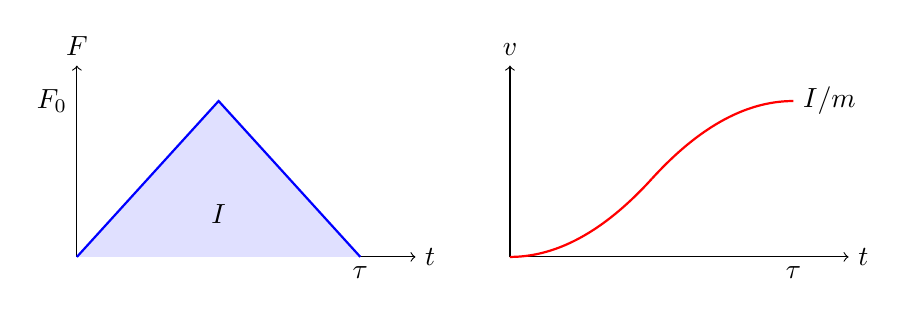
\begin{tikzpicture}[x=1cm,y=.9cm]
\draw[->](0,0)--(4.3,0)node[right]{$t$};\draw[->](0,0)--(0,2.7)node[above]{$F$};
\fill[blue!12](0,0)--(1.8,2.2)--(3.6,0)--cycle;\draw[blue,thick](0,0)--(1.8,2.2)--(3.6,0);
\node[left]at(0,2.2){$F_0$};\node[below]at(3.6,0){$\tau$};\node at(1.8,.6){$I$};
\begin{scope}[xshift=5.5cm]\draw[->](0,0)--(4.3,0)node[right]{$t$};\draw[->](0,0)--(0,2.7)node[above]{$v$};
\draw[red,thick,domain=0:1.8,samples=50]plot(\x,{2.2*\x*\x/6.48});\draw[red,thick,domain=1.8:3.6,samples=50]plot(\x,{2.2*(1-(3.6-\x)^2/6.48)});
\node[right]at(3.6,2.2){$I/m$};\node[below]at(3.6,0){$\tau$};\end{scope}
\end{tikzpicture}}



\par\medskip\Needspace{4\baselineskip}\noindent\textbf{以末速率计算总功并检查量纲}\par\nobreak
脉冲结束时质点质量不变，初动能为零，故总功可以通过末速度直接求出。代入$v=F_0\tau/(2m)$时，应平方整个分式：$mv^2/2=(m/2)F_0^2\tau^2/(4m^2)$，化简后得到下面的结果。

接着按图\ref{fig:em3:example:7:p}以相同末态应用动能定理，
\[\boxed{W=\tfrac12mv^2=F_0^2\tau^2/(8m)}.\]
若直接积分功率，利用 $F(t)\dd t=m\dd v$ 换元，时刻端点 $0,\tau$ 对应速度端点 $0,F_0\tau/(2m)$，得到
\[
W=\int_0^\tau F(t)v(t)\dd t
=m\int_0^{F_0\tau/(2m)}v\,\dd v
=m[v^2/2]_0^{F_0\tau/(2m)}
=\frac{F_0^2\tau^2}{8m}.
\]
冲量单位为$\mathrm{N\,s}$，功为$\mathrm{N\,m}$，量纲也能阻止把两种面积混同。\end{solution}
\begin{question}\begin{example}[竖直圆轨道上的摩擦功]\label{em3:example:8}
质量$m$的小车沿固定竖直圆轨道内侧以恒定速率$v$从最低点到最高点。半径$R$，动摩擦因数$\mu$，且$v^2\ge gR$保证保持内侧接触。驱动力沿切向，求摩擦功。
\end{example}
\fig{fig:em3:example:8:s}{题设：竖直圆轨道上的摩擦功}{\begin{tikzpicture}[scale=.9]\draw[world](2,0)circle(1.7);\fill(2,-1.7)circle(.09)node[below]{$A$};\fill(2,1.7)circle(.09)node[above]{$B$};\draw[flow](3.9,-.6)arc(-20:30:1.8);\node at(2.5,-.7){$R$};\end{tikzpicture}}
\end{question}
\begin{solution}\textbf{由恒速圆周运动求各处压力}\par\nobreak
按图\ref{fig:em3:example:8:s}从最低点起计转角$\theta$。径向向心方程为$N-mg\cos\theta=mv^2/R$，故$N=m(v^2/R+g\cos\theta)$。保持接触时$N\ge0$，其最小值在顶部，正给出题设速度条件。
\fig{fig:em3:example:8:p}{法向力进入摩擦力大小，切线微位移决定摩擦功的负号}{\begin{tikzpicture}

\coordinate(O)at(0,0);\coordinate(P)at(1.732,-1);\draw[world](0,0)circle(2);\draw[guide](0,-2)--(O)--(P);
\fill(P)circle(.08);\draw[force](P)--(.693,-.4)node[above]{$N$};\draw[force](P)--(1.732,-2.2)node[below]{$mg$};
\draw[force](P)--(1.132,-2.039)node[left]{$f=\mu N$};\draw[flow](P)--(2.332,.039)node[right]{$v,\ \dd s$};
\draw(0,-.7)arc(-90:-30:.7);\node at(.35,-.9){$\theta$};\node[left]at(0,-2){$A$};\node[above]at(0,2){$B$};
\node[align=left]at(5,.4){$N=m(v^2/R+g\cos\theta)$\\$\dd W_f=-\mu NR\dd\theta$};
\end{tikzpicture}}



\par\medskip\Needspace{4\baselineskip}\noindent\textbf{沿半周积分摩擦功}\par\nobreak
由图\ref{fig:em3:example:8:p}弧长微元$\dd s=R\dd\theta$，摩擦力始终逆运动方向，故
\[
W_f=-\int_0^\pi\mu NR\dd\theta
=-\mu m\int_0^\pi(v^2+gR\cos\theta)\dd\theta.
\]


\par\medskip\Needspace{4\baselineskip}\noindent\textbf{解释重力修正项为何相消}\par\nobreak
积分的两部分须分别代入上下限：
\[
\int_0^\pi v^2\dd\theta=v^2[\theta]_0^\pi=\pi v^2,
\qquad
\int_0^\pi gR\cos\theta\dd\theta=gR[\sin\theta]_0^\pi=0.
\]
所以$\boxed{W_f=-\pi\mu mv^2}$。消去的是重力对法向压力修正的积分，并不是球在升高过程中重力不做功；重力本身的功仍为$-2mgR$。

重力项在半周积分为零，但摩擦力本身并不恒定。小车动能不变，驱动力功必须补偿重力势能增加$2mgR$以及上述摩擦耗散。\end{solution}
\begin{question}\begin{example}[动滑轮拉力的瞬时功率]\label{em3:example:9}
水平物块与轻动滑轮固定连接。轻绳一端固定于右侧墙面，另一端受恒拉力$F$，该自由绳段与向右水平方向成$60^\circ$；靠墙固定段水平。物块向右速度为$v$。求外拉力的瞬时功率。
\end{example}
\fig{fig:em3:example:9:s}{题设：动滑轮拉力的瞬时功率}{\begin{tikzpicture}[scale=.9]\draw[world](0,0)rectangle(1,.8);\draw[world](1,.4)--(2,.4);\draw[world](2,.4)circle(.22);\draw[world](2,.18)--(4,.18);\draw[world](4,-.2)--(4,2.2);\draw[world](2,.62)--(2.8,2);\draw[flow](2.8,2)--(3.2,2.69)node[right]{$F$};\draw[flow](.2,1.2)--(1.3,1.2)node[above]{$v$};\node at(2.7,.9){$60^\circ$};\end{tikzpicture}}
\end{question}
\begin{solution}\textbf{计算两段绳张力对动滑轮的功率}\par\nobreak
图\ref{fig:em3:example:9:s}两段绳张力均为$F$，对动滑轮的水平合力为$F+F\cos60^\circ=3F/2$。滑轮与物块一起水平移动，所以这两个张力对动滑轮的功率和为$\boxed{P=3Fv/2}$。
\fig{fig:em3:example:9:p}{动滑轮的虚位移缩短两段绳，自由端须补足相同总长度}{\begin{tikzpicture}

\coordinate(C)at(0,0);\draw[world](C)circle(.35);\draw[force](0,-.35)--(2,-.35)node[right]{$F$};
\draw[force](-.303,.175)--(.697,1.907)node[above]{$F$};\draw[guide](-.303,.175)--(1.4,.175);
\draw(.397,.175)arc(0:60:.7);\node at(.65,.6){$60^\circ$};
\draw[flow](0,-1)--(1.4,-1)node[right]{$v,\ \dd x$};
\begin{scope}[xshift=4.4cm]\draw[guide](0,0)--(2,0);\draw[guide](0,0)--(1,1.732);\draw[flow](0,0)--(.7,0)node[midway,below]{$\dd x$};
\draw[dim](0,.35)--(.175,.653)node[left]{$\dd x\cos60^\circ$};
\draw[guide](.7,0)--(.175,.303);\node[align=left]at(1.3,-1.2){$\dd s=\dd x+\dd x\cos60^\circ$\\$P=F\dot s$};\end{scope}
\end{tikzpicture}}



\par\medskip\Needspace{4\baselineskip}\noindent\textbf{把滑轮功率与自由端输入联系起来}\par\nobreak
这个合功率通过轻绳等于自由端外力输入的功率，因为绳无质量、无伸长储能、轮轴无损耗。不能直接写$Fv$，因为$v$是动滑轮与物块的速度，自由端沿受力方向的速度一般不同；下面用图中的两绳段分别微分来确定它。



\par\medskip\Needspace{4\baselineskip}\noindent\textbf{用绳长微分核验自由端速度}\par\nobreak
也可由图\ref{fig:em3:example:9:p}的绳长微分核验。动滑轮向右位移$\dd x$，水平固定段缩短$\dd x$，斜段因轮端运动缩短$\dd x\cos60^\circ$，因此自由端必须沿绳增加长度$\dd s=(1+\cos60^\circ)\dd x$。于是$P=F\dd s/\dd t=3Fv/2$。角度随运动变化时，这个关系是该瞬间的微分关系。\end{solution}
\begin{question}\begin{example}[悬垂长绳与分段粗糙桌面]\label{em3:example:10}
长$6L$、质量$6m$的匀质绳，连接质量$M$的物块。水平路径$AB=BC=CD=DE=L$，绳从$E$处垂下，初始物块在$A$，悬垂绳长$2L$。$AB$光滑，$BE$有滑动摩擦，绳与桌面无摩擦，桌高大于$6L$。释放后物块最终停在$C$。求到$B$的速度及摩擦因数；若改为$21m/(4M)$求首次停止点；是否可选择摩擦因数使物块从$A$一路到$E$才首次停止？
\end{example}
\fig{fig:em3:example:10:s}{绳长6L中初始水平部分为4L，悬垂部分为2L}{\begin{tikzpicture}

\draw[world](-.4,0)--(4,0)--(4,-2.5);\draw[very thick](0,.1)--(4,.1)--(4,-1.9);
\filldraw[fill=white](-.25,.1)rectangle(.25,.6);\node at(0,.35){$M$};
\draw[brown,very thick](1,-.05)--(4,-.05);\node at(2.5,.9){物块与桌面有摩擦，绳无摩擦};
\foreach \xx/\lab in {0/A,1/B,2/C,3/D,4/E}{\draw(\xx,0)--(\xx,-.12);\node[below]at(\xx,-.15){$\lab$};}
\draw[dim](0,-.7)--(1,-.7)node[midway,below]{$L$};\draw[dim](4.6,.1)--(4.6,-1.9)node[midway,right]{$2L$};
\draw[flow](.25,.4)--(.9,.4)node[midway,above]{$s$};
\end{tikzpicture}}
\end{question}
\begin{solution}\textbf{把悬垂长度变化转为重力功}\par\nobreak
设图\ref{fig:em3:example:10:s}物块向右移动$s$，绳线密度为$m/L$，悬垂长度变成$2L+s$。以桌面为零势面、向下距离为 $y$，悬垂长度为 $h$ 时
\[
U(h)=-\frac{mg}{L}\int_0^h y\,\dd y
=-\frac{mg}{L}[y^2/2]_0^h
=-\frac{mg}{2L}h^2.
\]
初末分别取 $h=2L$ 与 $2L+s$，绳的重力势能减少
\[W_g=\frac{mg}{2L}\bigl[(2L+s)^2-(2L)^2\bigr]=mg\left(2s+\frac{s^2}{2L}\right).\]
系统总动能为$K=\tfrac12(M+6m)v^2$。在$B$处$s=L$且尚无摩擦功，故
\[\boxed{v_B=\sqrt{5mgL/(M+6m)}}.\]
从$A$到$B$，粗糙段尚未开始，因此只累计悬垂绳势能减少；从$B$继续到$s$时，物块相对固定桌面的粗糙滑程才是$s-L$。所以粗糙段一般能量式为$\tfrac12(M+6m)v^2=mg(2s+s^2/2L)-\mu Mg(s-L)$，这也是后面各次选根的共同依据。



\par\medskip\Needspace{4\baselineskip}\noindent\textbf{用到C的停止条件确定摩擦因数}\par\nobreak
在$C$处$s=2L$且$K=0$，所以$6mgL-\mu MgL=0$，得到$\boxed{\mu=6m/M}$。
\fig{fig:em3:example:10:p}{总势能降低由新、旧悬垂绳段的重心变化确定}{\begin{tikzpicture}

\foreach \xx/\len/\lab in {0/2/初始,4/3.2/向右移动s后}{\begin{scope}[xshift=\xx cm]
\draw[world](-1,0)--(1.5,0);\draw[very thick](-.5,.08)--(1.2,.08)--(1.2,-\len);
\draw[dim](1.8,0)--(1.8,-\len);\node at(.3,.7){\lab};\end{scope}}
\fill(1.2,-1)circle(.05)node[left]{$C_0$};\fill(5.2,-1.6)circle(.05)node[left]{$C_s$};
\node[right]at(1.8,-1){$2L$};\node[right]at(5.8,-1.6){$2L+s$};
\node[align=center]at(2.8,-4){$U_0=-\frac{mg}{2L}(2L)^2$\qquad$U_s=-\frac{mg}{2L}(2L+s)^2$};
\end{tikzpicture}}



\par\medskip\Needspace{4\baselineskip}\noindent\textbf{改变摩擦因数时取第一个可达零点}\par\nobreak
图\ref{fig:em3:example:10:p}给出重力功$W_g=U_0-U_s$。再令$z=s/L$，粗糙段有$K/(mgL)=2z+z^2/2-(\mu M/m)(z-1)$。改用$\mu'=21m/(4M)$，展开并分解：
\[
\frac{K}{mgL}=\frac{z^2}{2}-\frac{13z}{4}+\frac{21}{4}
=\frac{(2z-7)(z-3)}4
=\frac12(z-3)\left(z-\frac72\right).
\]
如图\ref{fig:em3:example:10:roots}，从$B$的$z=1$向右运动，首先遇到的零点为$z=3$，故首次停在$\boxed{D}$；另一根$z=7/2$在中间负动能区域之后，不可到达。此处悬垂重力$5mg$小于$\mu'Mg=5.25mg$，若最大静摩擦不小于动摩擦，则可保持停止。

\fig{fig:em3:example:10:roots}{放大首次零点附近；虚线负动能段不属于实际运动}{\begin{tikzpicture}

\begin{scope}[xshift=-5cm,x=2cm,y=8cm]\draw[axis](2.5,0)--(3.9,0)node[right]{$z=s/L$};\draw[axis](2.5,-.05)--(2.5,.18)node[above]{$K/(mgL)$};
\draw[blue,thick,domain=2.5:3,samples=40]plot(\x,{.5*(\x-3)*(\x-3.5)});
\draw[blue,dashed,domain=3:3.7,samples=60]plot(\x,{.5*(\x-3)*(\x-3.5)});
\foreach \xx in {3,3.5}{\fill(\xx,0)circle(.02cm);\node[above]at(\xx,0){$\xx$};}
\node[below]at(3.2,-.04){$K<0$};\end{scope}
\begin{scope}[xshift=1cm,x=1.8cm,y=4cm]\draw[axis](2.2,0)--(4.3,0)node[right]{$z$};\draw[axis](2.2,-.26)--(2.2,.22)node[above]{$K/(mgL)$};
\draw[red,thick,domain=2.2:2.666667,samples=40]plot(\x,{.5*(\x-8/3)*(\x-4)});
\draw[red,dashed,domain=2.666667:4.1,samples=60]plot(\x,{.5*(\x-8/3)*(\x-4)});
\node[above]at(2.666667,0){$8/3$};\node[above]at(4,0){$4$};\node at(3.25,-.08){$K<0$};\end{scope}
\node at(1.4,-1.4){$\mu M/m=21/4$，先停在$D$};\node at(7,-1.4){$\mu M/m=16/3$，不能到$E$};
\end{tikzpicture}}



\par\medskip\Needspace{4\baselineskip}\noindent\textbf{排除能量等式成立却无法到达E的根}\par\nobreak
若强令$E$处$z=4$为零，将其代入一般能量式，有$0=8+8-3\mu M/m$，解得$\mu=16m/(3M)$。再检查途中动能：
\[
\frac{K}{mgL}=\frac{z^2}{2}-\frac{10z}{3}+\frac{16}{3}
=\frac{(3z-8)(z-4)}6
=\frac12\left(z-\frac83\right)(z-4).
\]
在$z=8/3$就先停住，不能穿过负动能区到$E$。因此不存在所问的摩擦因数。只检查$E$处的能量等式会产生一个不能实现的解。\end{solution}
\begin{question}\begin{example}[船上抛球与内力做功]\label{em3:example:11}
人和船总质量$M$，另有质量$m$的球，最初共同以$v$运动。球以相对抛球后船的速度$u$水平抛出，分别沿船前进方向与反方向。忽略水阻，求系统所需增加的机械能，并求球和船各自的动能变化。
\end{example}
\fig{fig:em3:example:11:s}{抛球前人、船、球具有同一地面速度}{\begin{tikzpicture}

\draw[blue](-.5,0)--(5.5,0);\draw[world](0,.5)--(.5,0)--(4.5,0)--(5,.5)--cycle;
\fill(2,1.6)circle(.13);\draw[world](2,1.45)--(2,.5) (1.5,.5)--(2,1)--(2.5,.5) (2,1.2)--(2.7,1.2);
\fill(2.9,1.2)circle(.1)node[right]{$m$};\node at(1,.7){$M$};\draw[flow](.7,2.1)--(2.4,2.1)node[midway,above]{$v$};
\node[right]at(4.5,1.6){$u=|v_b-V|$};
\end{tikzpicture}}
\end{question}
\begin{solution}\textbf{用地面动量与相对速度求两个末速度}\par\nobreak
设抛球方向符号为$\sigma=\pm1$。按图\ref{fig:em3:example:11:s}在地面系写$(M+m)v=MV+m(V+\sigma u)$，所以船速$V=v-\sigma mu/(M+m)$，球速$v_b=v+\sigma Mu/(M+m)$。
\fig{fig:em3:example:11:p}{同一速度轴上比较前抛与后抛；两部分的动量增量相反}{\begin{tikzpicture}

\draw[axis](0,2)--(6.5,2)node[right]{速度};\draw[axis](0,0)--(6.5,0)node[right]{速度};
\draw[guide](3,-.5)--(3,2.7);\node[above]at(3,2.7){初速$v$};
\fill(1.8,2)circle(.06)node[below]{$V$};\fill(5.1,2)circle(.06)node[below]{$v_b$};
\draw[flow](3,2.5)--(1.8,2.5);\draw[flow](3,2.5)--(5.1,2.5);\node[left]at(0,2){前抛$\sigma=+1$};
\fill(4.2,0)circle(.06)node[below]{$V$};\fill(.9,0)circle(.06)node[below]{$v_b$};
\draw[flow](3,.5)--(4.2,.5);\draw[flow](3,.5)--(.9,.5);\node[left]at(0,0){后抛$\sigma=-1$};
\node at(3.2,-1.2){$M(V-v)=-m(v_b-v)$};
\end{tikzpicture}}



\par\medskip\Needspace{4\baselineskip}\noindent\textbf{分别展开球和船的动能变化}\par\nobreak
例如球的动能差展开为$\Delta K_b=(m/2)[(v+\sigma Mu/(M+m))^2-v^2]$，其中$\sigma^2=1$，故交叉项与$u^2$项分别保留。对船作同样展开，交叉项大小相等、符号相反；只有相加后才能消去整体平移速度$v$。

代入图\ref{fig:em3:example:11:p}各部分动能，分别得到
\[\begin{aligned}\Delta K_b&=\sigma\frac{mM}{M+m}vu+\frac{mM^2}{2(M+m)^2}u^2,\\\Delta K_M&=-\sigma\frac{mM}{M+m}vu+\frac{Mm^2}{2(M+m)^2}u^2.\end{aligned}\]


\par\medskip\Needspace{4\baselineskip}\noindent\textbf{合并为系统需要增加的机械能}\par\nobreak
相加后含$v$项抵消，故人的肌肉对机械运动输入的总能量为
\[\boxed{\Delta K=\tfrac12\frac{mM}{M+m}u^2},\]
两种方向相同。若$m=1\,\mathrm{kg},u=4\,\mathrm{m/s}$，得到$8M/(M+1)\,\mathrm J$，大船极限趋于$8\,\mathrm J$。船与人的动能变化可正可负，但不应把球的动能增加单独当作人的全部内力功。\end{solution}
\begin{question}\begin{example}[喷漆装置的理想功率]\label{em3:example:12}
静止喷漆装置把密度$\rho$的油漆从面积$S$的喷口以速率$v$喷出。入口油漆速度可忽略，出、入口高度相同，忽略粘滞和其他损失，求最低机械功率。
\end{example}
\fig{fig:em3:example:12:s}{题设：喷漆装置的理想功率}{\begin{tikzpicture}[scale=.9]\draw[world](0,-.5)rectangle(2,1);\draw[world](2,0)--(2.7,0)--(2.7,.5)--(2,.5);\draw[flow](2.9,.25)--(5.3,.25)node[above]{$v,S$};\node at(1,.25){$\rho$};\end{tikzpicture}}
\end{question}
\begin{solution}\textbf{由喷口面积与流速求质量流量}\par\nobreak
图\ref{fig:em3:example:12:s}单位时间喷出体积$Sv$，质量流量为$\dot m=\rho Sv$。每单位质量的动能增加为$v^2/2$，故
\[\boxed{P_{\min}=\frac12\dot m v^2=\frac12\rho Sv^3}.\]
\fig{fig:em3:example:12:p}{同一时间内喷出质量为密度乘射流微柱体积}{\begin{tikzpicture}[scale=.9]
\draw[thick](0,-1)--(0,1)--(2,1)--(3,.4)--(5,.4) (0,-1)--(2,-1)--(3,-.4)--(5,-.4);
\fill[blue!15](5,-.4)rectangle(6.5,.4);\draw[dashed](5,-.6)--(5,.6) (6.5,-.6)--(6.5,.6);
\draw[->,blue,thick](4.7,.9)--(6.5,.9)node[midway,above]{$v$};\draw[<->](5,-.9)--(6.5,-.9)node[midway,below]{$v\dd t$};
\node at(1,0){储液};\node[right]at(6.8,0){$S$};\node at(3,-1.8){$\dd m=\rho Sv\dd t,\quad\dd K=\tfrac12v^2\dd m$};\end{tikzpicture}}



\par\medskip\Needspace{4\baselineskip}\noindent\textbf{对同一时间喷出的流体计算动能增量}\par\nobreak
更直接地，在$\dd t$内喷出$\dd m=\rho Sv\dd t$，所需最低功$\dd W=(v^2/2)\dd m$，两边除以$\dd t$得到输入功率。这里计算的是进入、离开装置的油漆动能流，不是固定喷嘴本身的动能变化。



\par\medskip\Needspace{4\baselineskip}\noindent\textbf{区分射流能量流与静止喷嘴的受力功率}\par\nobreak
图\ref{fig:em3:example:12:p}把同一时间内的入、出流体分开，输入的压力功转为射流动能。喷嘴受到的反冲力为$\rho Sv^2$，但喷嘴静止，其位移为零；不能用“反冲力乘出流速度”计算喷嘴受力的功率。实际装置若存在效率$\eta<1$，所需输入功率应为$P_{\min}/\eta$。\end{solution}
\begin{question}\begin{example}[理想虹吸的排水时间]\label{em3:example:13}
很大的平底水槽装有$4\,\mathrm{kg}$的水，水深相对出口落差可忽略。虹吸管出口比槽底低$h=0.8\,\mathrm m$，截面积$S=0.01\,\mathrm{cm^2}$。忽略阻力，取$g=10\,\mathrm{m/s^2}$，求排空所需时间。
\end{example}
\fig{fig:em3:example:13:s}{题设：理想虹吸的排水时间}{\begin{tikzpicture}[scale=.9]\draw[world](0,2)--(0,1)--(2.5,1)--(2.5,2);\draw[guide](0,1.4)--(2.5,1.4);\draw[very thick](1.6,1.3)--(1.6,2.4)..controls(2,2.8)and(3,2.8)..(3.2,2.3)--(3.2,-.4);\draw[flow](3.2,-.4)--(3.2,-1);\draw[dim](4,-.4)--(4,1)node[midway,right]{$h$};\end{tikzpicture}}
\end{question}
\begin{solution}\textbf{由液面与出口的能量关系确定流速}\par\nobreak
取图\ref{fig:em3:example:13:s}沿管流动的一小团水。自由液面与出口均为大气压，大水槽液面速度可忽略，每单位质量下降$h$所减少的重力势能转为出口动能：$gh=v^2/2$，所以$v=\sqrt{2gh}=4\,\mathrm{m/s}$。
\fig{fig:em3:example:13:p}{沿流线比较自由液面与出口，压强相同而高度不同}{\begin{tikzpicture}

\draw[world](0,2.9)--(0,1.7)--(3,1.7)--(3,2.9);\fill[blue!8](0,1.7)rectangle(3,2.1);\draw[blue](0,2.1)--(3,2.1);
\draw[very thick](2,1.9)--(2,3.4)arc(180:0:.8)--(3.6,-.4);\draw[flow](3.6,-.4)--(3.6,-1.1)node[right]{$v$};
\fill(.7,2.1)circle(.05)node[above]{$A$};\fill(3.6,-.4)circle(.05)node[left]{$B$};
\draw[dim](4.5,1.7)--(4.5,-.4)node[midway,right]{$h$};\draw[guide](3,1.7)--(4.7,1.7);
\node[align=left]at(7,2.5){$p_A=p_B=p_{\rm atm}$\\$v_A\simeq0$\\$y_A-y_B\simeq h$};
\node at(2.2,-1.7){$\dot m=\rho Sv,\qquad T=M_{\text{水}}/\dot m$};
\end{tikzpicture}}



\par\medskip\Needspace{4\baselineskip}\noindent\textbf{统一面积、体积和质量流量的单位}\par\nobreak
单位换算须先平方长度单位：$1\,\mathrm{cm^2}=10^{-4}\,\mathrm{m^2}$，所以$0.01\,\mathrm{cm^2}=10^{-6}\,\mathrm{m^2}$。总水体积为$4/1000=0.004\,\mathrm{m^3}$；用它除以体积流量，与用总质量除以质量流量应得到同一时间。



\par\medskip\Needspace{4\baselineskip}\noindent\textbf{由恒定流量求排水时间并说明近似}\par\nobreak
按图\ref{fig:em3:example:13:p}，$S=10^{-6}\,\mathrm{m^2}$，体积流量$Q=Sv=4\times10^{-6}\,\mathrm{m^3/s}$，质量流量$\rho Q=0.004\,\mathrm{kg/s}$，因此
\[\boxed{T=4/0.004=1000\,\mathrm s}.\]
落差近似不变使流量近似恒定。虹吸最高处的压强还需足够高以免气化，题中默认虹吸已经建立并能维持。\end{solution}
\begin{question}\begin{example}[均匀链条越过半圆拱]\label{em3:example:14}
长$\pi R$、质量$m$的均匀链条原来平铺在水平面上，以初速$v_0$被送入固定光滑半圆拱形导槽。导槽两端与水平面等高、半径$R$，能从两侧约束链条且无摩擦。求能越过拱的临界初速，并区分临界值与有限时间越过条件。
\end{example}
\fig{fig:em3:example:14:s}{题设：均匀链条越过半圆拱}{\begin{tikzpicture}[scale=.9]\draw[world](-2,0)--(0,0);\draw[world](0,0)arc(180:0:2);\draw[world](4,0)--(6,0);\draw[very thick](-2,.1)--(0,.1);\draw[flow](-2,.7)--(-.5,.7)node[above]{$v_0$};\draw[dim](2,0)--(2,2)node[midway,right]{$R$};\end{tikzpicture}}
\end{question}
\begin{solution}\textbf{积分链条各微段的高度求最高势能}\par\nobreak
按图\ref{fig:em3:example:14:s}导槽约束只改变运动方向，不做功，链条各部分速率相同。链长恰等于半圆弧长，全链都在拱上时质心最高。取从左端起的角度$0\le\phi\le\pi$，高度$y=R\sin\phi$，线密度$\lambda=m/(\pi R)$，故该状态势能
\[
U_{\max}=\lambda gR^2\int_0^\pi\sin\phi\,\dd\phi
=\lambda gR^2[-\cos\phi]_0^\pi
=2\lambda gR^2=\frac{2mgR}{\pi}.
\]
\fig{fig:em3:example:14:p}{进入阶段势能递增；链条刚好铺满拱时质心最高}{\begin{tikzpicture}

\draw[world](0,0)arc(180:0:2);\draw[very thick](0,0)arc(180:0:2);\draw[guide](0,1.273)--(4,1.273);
\fill(2,1.273)circle(.06)node[left]{$C$};\node[above]at(2,2.5){$y_C=2R/\pi$};
\draw[guide](2,0)--(3.414,1.414);\draw[red,very thick](3.532,1.286)arc(40:50:2);
\node[right]at(3.6,1.7){$\dd m=\lambda R\dd\phi$};\draw[dim](4.5,0)--(4.5,1.414)node[midway,right]{$R\sin\phi$};
\begin{scope}[xshift=7cm]\draw[axis](0,0)--(4,0)node[right]{$\alpha$};\draw[axis](0,0)--(0,2.8)node[above]{$U$};
\draw[blue,thick,domain=0:180,samples=60]plot({\x/60},{1.2*(1-cos(\x))});
\draw[guide](0,2.4)--(3,2.4)--(3,0);\node[below]at(3,0){$\pi$};\node[left]at(0,2.4){$2mgR/\pi$};
\node at(1.8,-.7){$U=\lambda gR^2(1-\cos\alpha)$};\end{scope}
\end{tikzpicture}}



\par\medskip\Needspace{4\baselineskip}\noindent\textbf{由能量势垒求临界初速}\par\nobreak
图\ref{fig:em3:example:14:p}临界能量要求$mv_c^2/2=U_{\max}$，所以
\[\boxed{v_c=\sqrt{4gR/\pi}}.\]
由能量式，接入时全链总动能为$mv_0^2/2-\lambda gR^2(1-\cos\alpha)$。全链速率虽相同，各段高度却不同，因此不能把某个端点的上升高度乘整链重量。到$\alpha=\pi$时势能最高，且前面的积分可用$\int_0^\pi\sin\phi\dd\phi=2$逐步核验。



\par\medskip\Needspace{4\baselineskip}\noindent\textbf{检查更早势垒与临界到达时间}\par\nobreak
沿接入阶段，设进入弧角 $\alpha$，同一积分改取上限 $\alpha$，得到
\[
U(\alpha)=\lambda gR^2[-\cos\phi]_0^\alpha
=\lambda gR^2(1-\cos\alpha).
\]
因为 $U'(\alpha)=\lambda gR^2\sin\alpha>0$，进入时势能单调增加至全链在拱上；离开后则下降，因此没有更早的势垒。

严格要在有限时间越过，应取 $v_0>v_c$。等号时
$mv^2/2=U_{\max}-U=\lambda gR^2(1+\cos\alpha)$。
令 $\delta=\pi-\alpha$，则 $1+\cos\alpha=1-\cos\delta\simeq\delta^2/2$，从而
$v\simeq C\delta$，其中 $C=\sqrt{gR/\pi}$。
由 $R\dot\alpha=v$，在顶点附近从 $\delta=\varepsilon$ 到更小的 $\delta$ 所需时间为
\[
\Delta t\simeq\frac RC\int_\delta^\varepsilon\frac{\dd q}{q}
=\frac RC[\ln q]_\delta^\varepsilon
=\frac RC\ln(\varepsilon/\delta)\longrightarrow\infty.
\]
因此等号只给出临界下界。双侧导槽假设排除了单侧支承可能提前脱离的另一个限制。\end{solution}
\begin{question}\begin{example}[传送带加速物块的能量分配]\label{em3:example:15}
水平传送带由电机维持速率$U$，把质量$m$、初速度为零的物块轻放在带上，动摩擦因数$\mu$。求物块共速前的时间、物块位移、皮带相对滑程、电机为克服这项作用额外做的功及耗散。
\end{example}
\fig{fig:em3:example:15:s}{题设：传送带加速物块的能量分配}{\begin{tikzpicture}[scale=.9]\draw[world](0,0)rectangle(5,.3);\draw[world](.5,.3)rectangle(1.3,1);\node at(.9,.65){$m$};\draw[flow](2,-.5)--(4,-.5)node[above]{$U$};\end{tikzpicture}}
\end{question}
\begin{solution}\textbf{由加速过程求物块位移与带面滑程}\par\nobreak
图\ref{fig:em3:example:15:s}物块受向右摩擦$f=\mu mg$，加速度$\mu g$。从初速度零积分，
\[
v(t)=\int_0^t\mu g\dd\tau=\mu g[\tau]_0^t=\mu gt.
\]
共速条件$v(t_*)=U$给$t_*=U/(\mu g)$。再分别积分物块和带面的速度，
\begin{align*}
x&=\int_0^{t_*}\mu gt\dd t
=\mu g\left[\frac{t^2}{2}\right]_0^{t_*}
=\frac{\mu g}{2}\frac{U^2}{\mu^2g^2}=\frac{U^2}{2\mu g},\\
s_B&=\int_0^{t_*}U\dd t=U[t]_0^{t_*}
=Ut_* =\frac{U^2}{\mu g}.
\end{align*}
在$t<t_*$时$U-v(t)>0$，所用摩擦方向始终有效；相对滑程为$s_{\text{相}}=s_B-x=U^2/(2\mu g)$。
\fig{fig:em3:example:15:p}{速度图的两个三角形分别给出物块位移和相对滑程}{\begin{tikzpicture}

\draw[axis](0,0)--(5.1,0)node[right]{$t$};\draw[axis](0,0)--(0,3)node[above]{$v$};
\fill[blue!15](0,0)--(4,2.4)--(4,0)--cycle;\fill[red!12](0,0)--(0,2.4)--(4,2.4)--cycle;
\draw[world](0,0)--(4,2.4);\draw[blue,thick](0,2.4)--(4.7,2.4)node[right]{$U$};\draw[guide](4,0)--(4,2.4);
\node[below]at(4,0){$t_*$};\node[left]at(0,2.4){$U$};\node at(2.7,.6){$x$};\node at(1.3,1.8){$s_{\text{相}}$};
\begin{scope}[xshift=7cm]\draw[world](0,0)rectangle(2.6,.3);\draw[world](.4,.3)rectangle(1.2,1);\node at(.8,.65){$m$};
\draw[force](1.2,.65)--(2.4,.65)node[right]{$f$};\draw[force](1.2,-.5)--(0,-.5)node[left]{$f$};
\draw[flow](.4,1.4)--(2,1.4)node[right]{$v_m$};\draw[flow](.4,-1)--(2,-1)node[right]{$U$};
\node at(1.3,-1.7){$\dot Q=f(U-v_m)$};\end{scope}
\end{tikzpicture}}



\par\medskip\Needspace{4\baselineskip}\noindent\textbf{分别使用两个受力点的实际位移}\par\nobreak
由于滑动摩擦大小不变，物块自身获得的功是$fx$；皮带受到物块向左的等大摩擦，电机为补偿它，必须沿皮带运动距离$s_B$输入$fs_B$。两个功相减为$f(s_B-x)$，这正是相对滑动造成的耗散。



\par\medskip\Needspace{4\baselineskip}\noindent\textbf{核对电机输入、动能增加和耗散}\par\nobreak
按图\ref{fig:em3:example:15:p}电机为保持带速补偿的反作用力也为$f$，额外做功
\[\boxed{W_{\text{电机}}=fs_B=mU^2}.\]
物块动能增加
\[\boxed{\Delta K=mU^2/2},\]
耗散
\[\boxed{Q=fs_{\text{相}}=mU^2/2},\]
二者之和等于输入功。用物块位移算电机功会少一半，因为电机克服的是作用在运动带面上的阻力。\end{solution}
\begin{question}\begin{example}[摆球重力的最大功率]\label{em3:example:16}
长$\ell$的轻绳悬挂质量$m$小球，从水平位置静止释放。忽略阻力。以摆线与向下竖直方向夹角$\theta$表示位置，求下摆过程中重力功率的最大值及对应位置。
\end{example}
\fig{fig:em3:example:16:s}{摆长不变；下摆时速度沿切线，重力的切向分量为正}{\begin{tikzpicture}

\coordinate(O)at(0,3);\coordinate(P)at(2.298,1.072);\fill(O)circle(.05)node[above]{$O$};
\draw[guide](O)--(3,3);\fill(3,3)circle(.08)node[right]{释放};\draw[world](O)--(P)node[midway,above]{$\ell$};
\draw[guide](O)--(0,0);\draw[guide](3,3)arc(0:-90:3);\fill(P)circle(.08);
\draw(0,2.1)arc(-90:-40:.9);\node at(.35,1.9){$\theta$};
\draw[flow](P)--(1.655,.306)node[left]{$v$};\draw[force](P)--(2.298,-.25)node[right]{$mg$};
\end{tikzpicture}}
\end{question}
\begin{solution}\textbf{由下降高度与切向重力写出功率}\par\nobreak
图\ref{fig:em3:example:16:s}小球从水平位置下降$\ell\cos\theta$，能量给$v=\sqrt{2g\ell\cos\theta}$。重力沿速度方向的分量为$mg\sin\theta$，故$P=mg\sqrt{2g\ell}\sin\theta\sqrt{\cos\theta}$。
\fig{fig:em3:example:16:p}{精确函数c−c³的内部极值与两个端点共同确定最大功率}{\begin{tikzpicture}

\draw[axis](0,0)--(5.5,0)node[right]{$c=\cos\theta$};\draw[axis](0,0)--(0,3)node[above]{$P^2/(2m^2g^3\ell)$};
\draw[blue,thick,domain=0:1,samples=100]plot({5*\x},{6*(\x-\x*\x*\x)});
\draw[guide](2.887,0)--(2.887,2.309)--(0,2.309);\fill(2.887,2.309)circle(.055);
\node[below]at(2.887,0){$1/\sqrt3$};\node[below]at(5,0){$1$};\node[left]at(0,2.309){$2/(3\sqrt3)$};
\draw[flow](.6,.8)--(1.8,.8)node[midway,above]{下摆};
\end{tikzpicture}}



\par\medskip\Needspace{4\baselineskip}\noindent\textbf{用余弦变量化为多项式极值}\par\nobreak
最大化$P^2$与最大化非负的$P$具有同一位置。令$c=\cos\theta\in[0,1]$，将$\sin^2\theta=1-c^2$代入，有
\[
\frac{P^2}{2m^2g^3\ell}=f(c)=c(1-c^2)=c-c^3,
\qquad f'(c)=1-3c^2.
\]
令$f'=0$，得$c=\pm1/\sqrt3$；负根不在物理区间内，只保留$c_*=1/\sqrt3$。



\par\medskip\Needspace{4\baselineskip}\noindent\textbf{比较内部极值与两个端点}\par\nobreak
按图\ref{fig:em3:example:16:p}，$f'$在$c<c_*$时为正、$c>c_*$时为负；又$f(0)=f(1)=0$，故$c_*$给全局最大值。代入计算
\[
f(c_*)=\frac1{\sqrt3}-\frac1{3\sqrt3}=\frac2{3\sqrt3}.
\]
再由$P\ge0$取平方根，所以
\[\boxed{P_{\max}=mg\sqrt{2g\ell}\sqrt{\frac{2}{3\sqrt3}},\quad\cos\theta=\frac1{\sqrt3}}.\]
最低点速度最大，但重力与速度垂直，功率反而为零。绳张力在整个理想摆动中都不做功，不能用$Tv$充当其功率。\end{solution}
\begin{question}\begin{example}[固定球面上的脱离与落点]\label{em3:example:17}
小质点从固定光滑球面顶端由微小扰动滑下，球半径$R$，球心位于水平地面上。求脱离球面的位置与速度，并用抛体方程表示落地点。忽略空气阻力。
\end{example}
\fig{fig:em3:example:17:s}{题设：固定球面上的脱离与落点}{\begin{tikzpicture}[scale=.9]\draw[world](-2,0)arc(180:0:2);\draw[world](-2.7,0)--(4,0);\fill(0,2)circle(.08);\draw[guide](0,0)--(0,2) (0,0)--(1.4,1.428);\draw(0,.7)arc(90:45:.7);\node at(.3,.9){$\theta$};\end{tikzpicture}}
\end{question}
\begin{solution}\textbf{联立能量和非负支持力条件求脱离}\par\nobreak
按图\ref{fig:em3:example:17:s}从顶端计转角$\theta$，能量式$v^2=2gR(1-\cos\theta)$，径向式$mg\cos\theta-N=mv^2/R$。支持力只能非负，首次$N=0$给
\[\boxed{\cos\theta_d=2/3,\ v_d=\sqrt{2gR/3}}.\]

\fig{fig:em3:example:17:p}{先沿球面到脱离点，再用切线速度的两个分量求抛体落点}{\begin{tikzpicture}

\draw[world](-2,0)arc(180:0:2);\draw[world](-2.7,0)--(3.2,0);\coordinate(D)at(1.490712,1.333333);
\draw[guide](0,0)--(D);\fill(D)circle(.075)node[above right]{$D$};\node[below]at(0,0){$O$};
\draw[flow](D)--(2.290712,.438906)node[right]{$v_d$};
\draw[red,thick,domain=0:.98525345,samples=70]plot({1.490712+.76980036*\x},{1.333333-.86066297*\x-.5*\x*\x});
\fill(2.24916044,0)circle(.05)node[below]{$x_f$};
\begin{scope}[xshift=5cm]\draw[flow](0,1.4)--(.9,.394)node[below left]{$v_d$};
\draw[guide](0,1.4)--(.9,1.4)node[midway,above]{$2v_d/3$};
\draw[guide](.9,1.4)--(.9,.394)node[midway,right]{$-\sqrt5v_d/3$};
\node at(.5,2.5){脱离后$N=0$};\end{scope}
\end{tikzpicture}}



\par\medskip\Needspace{4\baselineskip}\noindent\textbf{由半径方向确定飞出速度分量}\par\nobreak
将能量速度代入径向式，$N=mg\cos\theta-2mg(1-\cos\theta)=mg(3\cos\theta-2)$。由顶端向下运动时余弦单调减小，第一次$N=0$为$\cos\theta=2/3$。速度方向沿半径$(\sin\theta,\cos\theta)$的右下切线$(\cos\theta,-\sin\theta)$，因此后面的两速度分量都有明确的几何依据。



\par\medskip\Needspace{4\baselineskip}\noindent\textbf{从脱离点切换到抛体运动并求落地根}\par\nobreak
在图\ref{fig:em3:example:17:p}取球心为原点，脱离点$(x_d,y_d)=(\sqrt5R/3,2R/3)$，沿右下切线飞出，速度分量为$(2v_d/3,-\sqrt5v_d/3)$。令$b=\sqrt5v_d/3>0$，后续竖直位置为$y=y_d-bt-gt^2/2$。落地条件$y=0$乘$2g$并配方，
\[
g^2t^2+2gbt=2gy_d,\qquad
(gt+b)^2=b^2+2gy_d.
\]
两根为$t=(-b\pm\sqrt{b^2+2gy_d})/g$。因为$y_d>0$，只有正号给正时间，故
\[
t_f=\frac{-\sqrt5v_d/3+\sqrt{5v_d^2/9+4gR/3}}{g},
\qquad \boxed{x_f=\frac{\sqrt5R}{3}+\frac{2v_d}{3}t_f}.
\]
能量式本身会允许球继续沿圆弧下降，但所需$N$变负时单侧球面无法维持约束，必须在此切换为抛体运动。\end{solution}
\begin{question}\begin{example}[不能定义单值势能的平面力场]\label{em3:example:18}
质点在平面力场$\bm F=(-ky,kx)$中沿半径$R$圆周绕原点逆时针一周，$k>0$。求该力做功，判断它是否为保守力，并讨论沿相反方向运动的功。
\end{example}
\fig{fig:em3:example:18:s}{力场沿以原点为圆心的圆周切向，方向始终逆时针}{\begin{tikzpicture}

\draw[world](0,0)circle(1.8);\draw[axis](-2.4,0)--(2.8,0)node[right]{$x$};\draw[axis](0,-2.3)--(0,2.6)node[above]{$y$};
\node[below left]at(0,0){$O$};\draw[dim](0,0)--(1.273,1.273)node[midway,below right]{$R$};
\draw[flow](2,0)arc(0:75:2);\foreach \ang in {0,90,180,270}{\draw[force]({1.8*cos(\ang)},{1.8*sin(\ang)})--++({.8*cos(\ang+90)},{.8*sin(\ang+90)});}
\node at(4.2,.5){$\bm F=(-ky,kx)$};
\end{tikzpicture}}
\end{question}
\begin{solution}\textbf{参数化圆周并写出位移微元}\par\nobreak
按图\ref{fig:em3:example:18:s}参数化$x=R\cos\phi,y=R\sin\phi$，逐项微分得到$\dd x=-R\sin\phi\dd\phi$、$\dd y=R\cos\phi\dd\phi$。因此$\dd\bm r=(-R\sin\phi,R\cos\phi)\dd\phi$；力也沿逆时针切向，大小为$kR$。
\fig{fig:em3:example:18:p}{在任意角度点积均为正；反向路径只改变位移微元方向}{\begin{tikzpicture}

\draw[world](0,0)circle(1.8);\coordinate(P)at(1.273,1.273);\draw[guide](0,0)--(P)node[midway,below]{$R$};\fill(P)circle(.065)node[right]{$P$};
\draw[force](P)--(.424,2.122)node[left]{$\bm F=kR\bm e_\phi$};
\draw[flow](1.556,1.556)--(.99,2.122)node[above right]{$\dd\bm r=R\dd\phi\bm e_\phi$};
\draw[axis](0,0)--(2.7,0)node[right]{$x$};\draw(.6,0)arc(0:45:.6);\node at(.8,.3){$\phi$};
\node[align=left]at(5,.5){逆时针：$\dd W=kR^2\dd\phi$\\顺时针：$\dd\phi<0$};
\end{tikzpicture}}



\par\medskip\Needspace{4\baselineskip}\noindent\textbf{利用切向力积分闭路功}\par\nobreak
图\ref{fig:em3:example:18:p}中，点积展开为
\[
\bm F\cdot\dd\bm r
=[(-kR\sin\phi)(-R\sin\phi)+(kR\cos\phi)(R\cos\phi)]\dd\phi
=kR^2\dd\phi.
\]
利用$\sin^2\phi+\cos^2\phi=1$后，被积函数为常量。逆时针一周对应$\phi:0\to2\pi$，故
\[
W=\int_0^{2\pi}\bm F\cdot\dd\bm r
=kR^2\int_0^{2\pi}\dd\phi
=kR^2[\phi]_0^{2\pi}=\boxed{2\pi kR^2}.
\]
闭合路径的非零功足以否定保守性，无需先猜势能函数。



\par\medskip\Needspace{4\baselineskip}\noindent\textbf{用闭路功判定保守性和反向功}\par\nobreak
图\ref{fig:em3:example:18:p}起点终点相同而功不为零，故不能用仅由位置决定的单值势能表示该力。顺时针一周则$W=-2\pi kR^2$。这也提醒，写$F_x=-\partial U/\partial x$时必须确认同一$U$还能同时满足其他分量，不能对每个分量各自积分后任意拼合。\end{solution}
